% Define
\documentclass{exam}


% Using Packages
\usepackage[a4paper, total={6in, 8in}]{geometry}
\usepackage{geometry}
\usepackage{graphicx}
\usepackage{amsmath}
\usepackage{amssymb}
\usepackage{parskip}
\usepackage{dsfont}
\usepackage[utf8]{inputenc}
\usepackage{pythonhighlight}


% Page Setting
\geometry{a4paper}

% Title
\title{Machine Learning Coursework}
\date{Monday 11th March, 2024}
\author{Khalid Belhadj S2233559}

% Document
\begin{document}
\maketitle

\newcommand{\hr}{\noindent\rule{\linewidth}{0.4pt}}

\begin{questions}
    % Question 1
    \question
    \begin{parts}
        \part % a

        % Convexity
        {
            Show that if a function $f$ is convex, then
            \begin{equation} \label{eq:ineq1}
                f(y) - f(x) - \nabla f(x)^\top(y - x) \leq  (\nabla f(y) - \nabla f(x))^\top(y - x)
            \end{equation}
            for any $x$ and $y$.

            \textbf{Solution.}

            A function $f$ is convex if
            \begin{equation} \label{eq:convex}
                f(\alpha x + (1 - \alpha)y) \leq \alpha f(x) + (1 - \alpha)f(y)
            \end{equation}
            for every $x, y$ and $0 \leq \alpha \leq 1$.

            We can use definition \eqref{eq:convex} to prove that if a function $f$ is convex, then (from lecture 7, slide 8)
            \begin{equation}
                f(x) \geq f(y) + \nabla f(y)^\top(x - y)
            \end{equation}

            \textbf{Proof.}

            \begin{align*}
                f(\alpha x + (1 - \alpha)y)                              & \leq \alpha f(x) + (1 - \alpha)f(y) \\
                f(\alpha x + (1 - \alpha)y) - (1 - \alpha)f(y)           & \leq \alpha f(x)                    \\
                f(\alpha x + (1 - \alpha)y) - f(y) + \alpha f(y)         & \leq \alpha f(x)                    \\
                \frac{f(\alpha x + (1 - \alpha)y) - f(y)}{\alpha} + f(y) & \leq f(x)                           \\
                \frac{f(\alpha x + y - \alpha y) - f(y)}{\alpha} + f(y)  & \leq f(x)                           \\
                f(y) + \nabla f(y)^\top(x - y)                           & \leq f(x)
            \end{align*}

            Starting with the left hand side of \eqref{eq:ineq1}, and substituting $f(x)$ for the right hand side of \eqref{eq:convex}
            \begin{align*}
                f(y) - f(x) - \nabla f(x)^\top(y - x) & \leq f(y) - (f(y) - \nabla f(y)^\top(x - y)) - \nabla f(x)^\top(y - x) \\
                                                      & =  - \nabla f(y)^\top(x - y) - \nabla f(x)^\top(y - x)                 \\
                                                      & =  \nabla f(y)^\top(y - x) - \nabla f(x)^\top(y - x)                   \\
                f(y) - f(x) - \nabla f(x)^\top(y - x) & \leq  (\nabla f(y) - \nabla f(x))^\top(y - x) \text{ Q.E.D.}
            \end{align*}
            Thus it is shown that if a function $f$ is convext, then the inequality \eqref{eq:ineq1} holds.
        }

        \hr

        % Cauchy-Schwarz
        {
            Remind yourself what Cauchy-Schwarz is. Show that if a function $f$ is convex, then
            \begin{equation} \label{eq:cauchy}
                f(y) - f(x) - \nabla f(x)^\top(y - x)  \leq \Vert \nabla f(y) - \nabla f(x) \Vert_2 \Vert y - x \Vert_2
            \end{equation}

            for any $x$ and $y$.

            \textbf{Solution.}

            The Cauchy-Schwarz inequality states that
            \begin{equation}
                \vert \bf{u}^\top \bf{v} \vert \leq \Vert \bf{u} \Vert \Vert \bf{v} \Vert
            \end{equation}

            It was previously shown that if $f$ is convex then
            \begin{align*}
                f(x) \geq f(y) + \nabla f(y)^\top(x - y)
            \end{align*}
            Similarly,
            \begin{align*}
                f(y) \geq f(x) + \nabla f(x)^\top(y - x)
            \end{align*}
            By adding both of these inequalities we get
            \begin{align*}
                f(x) + f(y) & \geq f(y) + \nabla f(y)^\top(x - y) + f(x) + \nabla f(x)^\top(y - x) \\
                0 & \geq\nabla f(y)^\top(x - y) + \nabla f(x)^\top(y - x) \\
                0 & \geq\nabla f(y)^\top(x - y) - \nabla f(x)^\top(x - y) \\
                0 & \geq (\nabla f(y) - \nabla f(x))^\top(x - y) \\
                0 & \leq (\nabla f(y) - \nabla f(x))^\top(y - x) \\
            \end{align*}
            Therefore, we know that
            \begin{align*}
                (\nabla f(y) - \nabla f(x))^\top(y - x) = \vert (\nabla f(y) - \nabla f(x))^\top(y - x) \vert \\
            \end{align*}

            Taking the right hand side of inequality \eqref{eq:ineq1}, we can apply the Cauchy-Schwarz inequality to get
            Using \eqref{eq:ineq1}, and applying the Cauchy-Schwarz inequality to the right hand side
            \begin{align*}
                f(y) - f(x) - \nabla f(x)^\top(y - x) & \leq (\nabla f(y) - \nabla f(x))^\top(y - x)                                    \\
                                                      & = \vert (\nabla f(y) - \nabla f(x))^\top(y - x) \vert                           \\
                                                      & \leq \Vert \nabla f(y) - \nabla f(x) \Vert_2 \Vert y - x \Vert_2 \text{ Q.E.D.}
            \end{align*}

            Therefore it is shown that if $f$ is convex, then \eqref{eq:cauchy} holds.
        }

        \hr

        % L-smooth
        {
            Show that if a function $f$ is convex and \emph{L}-smooth, then
            \begin{equation}\label{eq:l}
                f(y) \leq f(x) + \nabla f(x)^\top (y - x) + \emph{L}\Vert x - y \Vert ^2_2
            \end{equation}

            for any $x$ and $y$.


            \textbf{Solution.}

            A function is said to be \emph{L}-smooth if
            \begin{equation}
                \Vert \nabla f(x) - \nabla f(y) \Vert_2 \leq \emph{L} \Vert x - y \Vert_2
            \end{equation}

            Starting from inequality \eqref{eq:cauchy},
            \begin{align*}
                f(y) - f(x) - \nabla f(x)^\top(y - x) & \leq \Vert \nabla f(y) - \nabla f(x) \Vert_2 \Vert y - x \Vert_2                    \\
                                                      & = \emph{L} \Vert y - x \Vert_2 \Vert y - x \Vert_2                                  \\
                                                      & = \emph{L} \Vert y - x \Vert_2^2                                                    \\
                f(y)                                  & \leq f(x) + \nabla f(x)^\top(y - x) + \emph{L} \Vert y - x \Vert_2^2 \text{ Q.E.D.}
            \end{align*}
            Therefore it is shown that if $f$ is convex and \emph{L}-smooth, then \eqref{eq:l} holds.
        }

        \hr

        \part % b

        % Gradient descent
        {
            Given that gradient descent can be summerised as
            \begin{equation}
                x_t = x_{t-1} - \eta \nabla f(x_{t-1})
            \end{equation}
            show that
            \begin{equation}\label{eq:gd}
                f(x_{t - 1}) - f(x_t) \geq \eta_t(1 - \emph{L}\eta_t)\Vert \nabla f (x_{t - 1}) \Vert _2^2
            \end{equation}
            \textbf{Solution.}

            Using \eqref{eq:l}, we can plug in $x = x_{t - 1}$ and $y = x_t$
            \begin{align*}
                f(x_t)                  & \leq f(x_{t - 1}) + \nabla f(x_{t - 1})^\top (x_t - x_{t - 1}) + \emph{L}\Vert x_{t - 1} - x_t \Vert ^2_2                                                                       \\
                f(x_t)                  & \leq f(x_{t - 1}) + \nabla f(x_{t - 1})^\top (x_{t - 1} - \eta_t \nabla f(x_{t - 1}) - x_{t - 1}) + \emph{L}\Vert x_{t - 1} - x_{t - 1} + \eta_t \nabla f(x_{t - 1}) \Vert ^2_2 \\
                f(x_t)                  & \leq f(x_{t - 1}) + \nabla f(x_{t - 1})^\top (- \eta_t \nabla f(x_{t - 1})) + \emph{L}\Vert \eta_t \nabla f(x_{t - 1}) \Vert ^2_2                                               \\
                f(x_t)                  & \leq f(x_{t - 1}) - \eta_t \nabla f(x_{t - 1})^\top \nabla f(x_{t - 1}) +  \eta_t^2 \emph{L}\Vert \nabla f(x_{t - 1}) \Vert ^2_2                                                \\
                f(x_t)                  & \leq f(x_{t - 1}) - \eta_t \nabla \Vert f(x_{t - 1})\Vert ^2_2 + \eta_t^2 \emph{L}\Vert \nabla f(x_{t - 1}) \Vert ^2_2                                                          \\
                - f(x_{t - 1}) + f(x_t) & \leq  - \eta_t \nabla \Vert f(x_{t - 1})\Vert ^2_2 + \eta_t^2 \emph{L}\Vert \nabla f(x_{t - 1}) \Vert ^2_2                                                                      \\
                f(x_{t - 1}) - f(x_t)   & \geq  \eta_t \nabla \Vert f(x_{t - 1})\Vert ^2_2 - \eta_t^2 \emph{L}\Vert \nabla f(x_{t - 1}) \Vert ^2_2                                                                        \\
                f(x_{t - 1}) - f(x_t)   & \geq \eta_t(1 - \emph{L}\eta_t)\Vert \nabla f (x_{t - 1}) \Vert _2^2 \text{ Q.E.D.}
            \end{align*}
            Therefore it is shown that \eqref{eq:gd} holds.
        }

        \hr

        % Convergence
        {
            Consider $g(s) = s(1 - \emph{L}s)$. This is a concave parabola. Show that $g$ has a maximum of $\frac{1}{4\emph{L}}$ when $s = \frac{1}{2\emph{L}}$, and $g$ is 0 when $s = \frac{1}{\emph{L}}$.

            Finding the value of $s$ when $g(s)$ is 0

            \begin{align*}
                g(s)     & = s(1 - \emph{L}s)            \\
                0        & = s(1 - \emph{L}s)            \\
                s    = 0 & \text{ or } 1 - \emph{L}s = 0 \\
                1        & = \emph{L}s                   \\
                s        & = \frac{1}{\emph{L}}
            \end{align*}
            As shown above, $g(s)$ is 0 when $s = \frac{1}{\emph{L}}$, and when $s = 0$.

            Finding the first derivative of $g(s)$
            \begin{align*}
                \frac{\partial}{\partial s} (g(s)) & = \frac{\partial}{\partial s} \left( s(1 - \emph{L} s) \right)                                           \\
                                                   & = \frac{\partial}{\partial s} \left( s - \emph{L} s^2 \right)                                            \\
                                                   & = \frac{\partial}{\partial s} \left( s \right) - \frac{\partial}{\partial s} \left( \emph{L} s^2 \right) \\
                                                   & = 1 - 2\emph{L}s
            \end{align*}

            Finding the second derivative of $g(s)$
            \begin{align*}
                \frac{\partial^2}{\partial^2 s} (g(s)) & = \frac{\partial}{\partial s} \left(\frac{\partial}{\partial s} (g(s))\right)                       \\
                                                       & = \frac{\partial}{\partial s} \left(1 - 2\emph{L}s\right)                                           \\
                                                       & = \frac{\partial}{\partial s} \left(1 \right) - \frac{\partial}{\partial s} \left(2\emph{L}s\right) \\
                                                       & = -2\emph{L}
            \end{align*}

            To find the extrema of $g(s)$, we can set the first derivative to 0
            \begin{align*}
                0          & = 1 - 2\emph{L}s      \\
                2\emph{L}s & = 1                   \\
                s          & = \frac{1}{2\emph{L}}
            \end{align*}

            Given that $\emph{L} > 0$, we know that the second derivative $-2\emph{L}$ is negative, and therefore the extrema is a maximum. The find the maximum value of $g(s)$, we can plug in $s = \frac{1}{2\emph{L}}$ into $g(s)$
            \begin{align*}
                g\left(\frac{1}{2\emph{L}}\right) & = \frac{1}{2\emph{L}}\left(1 - \emph{L}\frac{1}{2\emph{L}}\right) \\
                                                  & = \frac{1}{2\emph{L}}\left(1 - \frac{1}{2}\right)                 \\
                                                  & = \frac{1}{4\emph{L}}
            \end{align*}

            Hence it is shown that $g$ has a maximum of $\frac{1}{4\emph{L}}$ when $s = \frac{1}{2\emph{L}}$, and $g$ is 0 when $s = \frac{1}{\emph{L}}$
        }

        \hr

        \part % c
        % Minimising g(s)
        {

            A function $f$ is said to be $\mu$-strongly convex if
            \begin{equation} \label{eq:mu}
                f(y) \geq f(x) + \nabla f(x) ^\top (y - x) + \frac{\mu}{2}\Vert y - x \Vert^2_2
            \end{equation}
            for any $x$ and $y$.

            Show that, for a particular $x$, the quadratic function on thr right hand side
            \begin{equation}\label{eq:g}
                g(z) = f(x) + \nabla f(x) ^\top (z - x) + \frac{\mu}{2}\Vert z - x \Vert^2_2
            \end{equation}
            is minimised when $z = x - \frac{1}{\mu}\nabla f(x)$.

            \textbf{Solution.}

            Finding the first partial derivative of $g$ with respect to $z$
            \begin{align*}
                \frac{\partial}{\partial z} \left(g(z)\right) & = \frac{\partial}{\partial z} \left(f(x) + \nabla f(x) ^\top (z - x) + \frac{\mu}{2}\Vert z - x \Vert^2_2\right)                                                                                 \\
                                                              & = \frac{\partial}{\partial z} \left(f(x)\right) + \frac{\partial}{\partial z}\left(\nabla f(x) ^\top (z - x)\right) + \frac{\partial}{\partial z}\left(\frac{\mu}{2}\Vert z - x \Vert^2_2\right) \\
                                                              & = \frac{\partial}{\partial z}\left(\nabla f(x) ^\top (z - x)\right) + \frac{\mu}{2}\frac{\partial}{\partial z}\left(\Vert z - x \Vert^2_2\right)                                                 \\
                                                              & = \frac{\partial}{\partial z}\left(\nabla f(x) ^\top z - \nabla f(x) ^\top x\right) + \frac{\mu}{2}2\left(z - x\right)                                                                           \\
                                                              & = \frac{\partial}{\partial z}\left(\nabla f(x) ^\top z \right) - \frac{\partial}{\partial z}\left(\nabla f(x) ^\top x\right) + \mu\left(z - x\right)                                             \\
                                                              & = \frac{\partial}{\partial z}\left(\nabla f(x) ^\top z \right)  + \mu z - \mu x                                                                                                                  \\
                                                              & = \nabla f(x)  + \mu z - \mu x
            \end{align*}

            To find the minimising $z$ value of $g(z)$, we must find the value of $z$ such that $\frac{\partial g}{\partial z} = 0$
            \begin{align*}
                0      & = \nabla f(x)  + \mu z - \mu x                \\
                -\mu z & = \nabla f(x)  - \mu x                        \\
                \mu z  & =  \mu x -\nabla f(x)                         \\
                z      & =  \frac{\mu x -\nabla f(x)}{\mu}             \\
                z      & =  x -\frac{1}{\mu}\nabla f(x) \text{ Q.E.D.}
            \end{align*}
        }

        \hr

        {
            Show that
            \begin{equation}\label{eq:min}
                f(y) \geq g(y) \geq \min_{z} g(z) = f(x) - \frac{1}{2\mu} \Vert \nabla f(x) \Vert^2_2
            \end{equation}

            \textbf{Solution.}

            Using \eqref{eq:g} as the definition of $g(z)$, $g(y)$ is
            \begin{equation}
                g(y) = f(x) + \nabla f(x) ^\top (y - x) + \frac{\mu}{2}\Vert y - x \Vert^2_2
            \end{equation}
            which is equivalent to the right hand side of \eqref{eq:mu}. Therefore, we know that $f(y) \geq g(y)$. By the definition of a minimiser, we know that
            \begin{equation}\label{eq:minimiser}
                g(y) \geq \min_{z} g(z)
            \end{equation}
            and the $z$ value which minimises $g(z)$ was found to be $z_{min} = x -\frac{1}{\mu}\nabla f(x)$. Therefore, we can find $\min_{z} g(z)$
            \begin{align*}
                \min_{z} g(z) & = g(z_{min})                                                                                                                \\
                              & = g\left(x -\frac{1}{\mu}\nabla f(x)\right)                                                                                 \\
                              & = f(x) + \nabla f(x) ^\top (x -\frac{1}{\mu}\nabla f(x) - x) + \frac{\mu}{2}\Vert x -\frac{1}{\mu}\nabla f(x) - x \Vert^2_2 \\
                              & = f(x) + \nabla f(x) ^\top (-\frac{1}{\mu}\nabla f(x)) + \frac{\mu}{2}\Vert -\frac{1}{\mu}\nabla f(x) \Vert^2_2             \\
                              & = f(x) + -\frac{1}{\mu}\nabla f(x) ^\top \nabla f(x) + \frac{\mu}{2 \mu^2}\Vert \nabla f(x) \Vert^2_2                       \\
                              & = f(x) + -\frac{1}{\mu} \Vert \nabla f(x) \Vert_2^2 + \frac{1}{2 \mu}\Vert \nabla f(x) \Vert^2_2                            \\
                              & = f(x) - \frac{1}{2 \mu}\Vert \nabla f(x) \Vert^2_2
            \end{align*}
            Therefore we can conclude that based on the working above, and \eqref{eq:minimiser} that
            \begin{equation}
                g(y) \geq \min_{z} g(z) = f(x) - \frac{1}{2 \mu}\Vert \nabla f(x) \Vert^2_2
            \end{equation}

            Using the fact that $f(y) \geq g(y)$, and g(y) $\geq \min_{z} g(z)$, we conclude that
            \begin{equation}
                f(y) \geq g(y) \geq \min_{z} g(z) = f(x) - \frac{1}{2\mu} \Vert \nabla f(x) \Vert^2_2
            \end{equation}
        }

        \hr

        % Minimising x^*
        {
            Choose $y = x^*$ where $x^*$ is the minimiser of $f$, and conclude that
            \begin{equation} \label{eq:x}
                f(x) - f(x^*) \leq \frac{1}{2\mu}\Vert \nabla f(x) \Vert_2^2
            \end{equation}

            \textbf{Solution.}

            From \eqref{eq:min}, we know that
            \begin{equation}
                f(y) \geq f(x) - \frac{1}{2\mu} \Vert \nabla f(x) \Vert^2_2
            \end{equation}
            Substituting $x^*$ for y, we get
            \begin{align*}
                f(x^*)        & \geq f(x) - \frac{1}{2\mu} \Vert \nabla f(x) \Vert^2_2          \\
                f(x^*) - f(x) & \geq  - \frac{1}{2\mu} \Vert \nabla f(x) \Vert^2_2              \\
                f(x)- f(x^*)  & \leq  \frac{1}{2\mu} \Vert \nabla f(x) \Vert^2_2 \text{ Q.E.D.}
            \end{align*}
        }

        \hr

        \part % d

        {
            We know that if we perform gradient descent on a \emph{L}-smooth function $f$ then
            \begin{equation}
                f(x_t) \leq f(x_{t - 1}) - \frac{1}{4\emph{L}} \Vert \nabla f(x_{t - 1}) \Vert_2^2
            \end{equation}
            We can subtract $f(x^*)$ from both sides to get
            \begin{equation}\label{eq:d-starter}
                f(x_t) - f(x^*) \leq f(x_{t - 1}) - f(x^*) - \frac{1}{4\emph{L}} \Vert \nabla f(x_{t - 1}) \Vert_2^2
            \end{equation}
            If we further assume that $f$ is $\mu$-strongly ocnvex, show that
            \begin{equation}\label{eq:d-conclusion}
                f(x_t) - f(x^*) \leq \left(1 - \frac{\mu}{1\emph{L}}\right)\left(f(x_{t - 1} - f(x^*))\right)
            \end{equation}

            \textbf{Solution.}

            Using \eqref{eq:x}, we can substitute $x = x_{t - 1}$ to get
            \begin{align*}
                f(x_{t - 1}) - f(x^*)        & \leq \frac{1}{2\mu}\Vert \nabla f(x_{t - 1}) \Vert_2^2 \\
                2 \mu(f(x_{t - 1}) - f(x^*)) & \leq \Vert \nabla f(x_{t - 1}) \Vert_2^2               \\
            \end{align*}
            Then, we can substitute the result above into \eqref{eq:d-starter} to get
            \begin{align*}
                f(x_t) - f(x^*) & \leq f(x_{t - 1}) - f(x^*) - \frac{1}{4\emph{L}} \Vert \nabla f(x_{t - 1}) \Vert_2^2         \\
                                & \leq f(x_{t - 1}) - f(x^*) - \frac{2\mu}{4\emph{L}} (f(x_{t - 1}) - f(x^*))                  \\
                                & \leq f(x_{t - 1}) - f(x^*) - \frac{\mu}{2\emph{L}} (f(x_{t - 1}) - f(x^*))                   \\
                                & \leq \left(1 - \frac{\mu}{1\emph{L}}\right)\left(f(x_{t - 1}) - f(x^*)\right) \text{ Q.E.D.}
            \end{align*}
        }

        \hr

        {
            Apply this result repeatedly, and conclude that
            \begin{equation}
                f(x_t) - f(x^*) \leq \left(1 - \frac{\mu}{2\emph{L}}\right)^t(f(x_0) - f(x^*))
            \end{equation}

            \textbf{Solution.}

            Starting with \eqref{eq:d-conclusion}, we can see that we can reapply the inequality on the right hand side
            \begin{align*}
                f(x_t) - f(x^*) & \leq \left(1 - \frac{\mu}{1\emph{L}}\right)\left(f(x_{t - 1}) - f(x^*)\right)                                                     \\
                f(x_t) - f(x^*) & \leq \left(1 - \frac{\mu}{1\emph{L}}\right)\left(\left(1 - \frac{\mu}{1\emph{L}}\right)\left(f(x_{t - 2}) - f(x^*)\right) \right) \\
                                & = \left(1 - \frac{\mu}{1\emph{L}}\right)^2\left(f(x_{t - 2}) - f(x^*)\right)                                                      \\
            \end{align*}
            Once we apply this recursive step $t$ times, we get that
            \begin{align*}
                f(x_t) - f(x^*) & \leq \left(1 - \frac{\mu}{1\emph{L}}\right)\left(\left(1 - \frac{\mu}{1\emph{L}}\right)\left(f(x_{t - 2}) - f(x^*)\right) \right)                                                     \\
                                & \leq \left(1 - \frac{\mu}{1\emph{L}}\right)\left(\left(1 - \frac{\mu}{1\emph{L}}\right)\left(\left(1 - \frac{\mu}{1\emph{L}}\left(f(x_{t - 2}) - f(x^*)\right) \right)\right) \right) \\
                                & \leq \left(1 - \frac{\mu}{1\emph{L}}\right)\left(\left(1 - \frac{\mu}{1\emph{L}}\right)\left(\left(1 - \frac{\mu}{1\emph{L}}\left(f(x_{t - 3}) - f(x^*)\right) \right)\right) \right) \\
                                & \vdots                                                                                                                                                                                \\
                f(x_t) - f(x^*) & \leq \left(1 - \frac{\mu}{2\emph{L}}\right)^t(f(x_0) - f(x^*))
            \end{align*}
        }

        \hr

        {
            In sum, this is the convergence rate if we run gradient descent with a constant step size of $\frac{1}{2\emph{L}}$ on an \emph{L}-smooth, $\mu$-strongly convex function.

            Is the convergence quadratic, linear, or sublinear?

            The convergence seems to be linear. if we take $c = f(x_0) - f(x^*)$, which is a constant since $x_0$ and $x^*$ are both constants, and $r = (1 - \frac{\mu}{2\emph{L}})$, we can see that it is of the form
            \begin{equation}
                f(x_t) - f(x^*) \leq xr^t
            \end{equation}
        }

        \hr

    \end{parts}

    \newpage
    % Question 2
    \question
    \begin{parts}
        \part % a

        % Max a b c d
        {
            Show that
            \begin{equation}
                \max(a + b, c + d) \leq \max(a, c) + \max(b, d)
            \end{equation}

            \textbf{Solution.}

            Given that
            \begin{equation*}
                a \leq \max(a, c), b \leq \max(b, d)
            \end{equation*}
            we can deduce that
            \begin{equation*}
                a + b \leq \max(a, c), b \leq \max(b, d)
            \end{equation*}
            By the same reasoning, we know that
            \begin{equation*}
                c \leq \max(a, c), d \leq \max(b, d)
            \end{equation*}
            which means that
            \begin{equation*}
                c + d \leq \max(a, c), b \leq \max(b, d)
            \end{equation*}
            Therefore,
            \begin{equation*}
                \max(a + b, c + d) \leq \max(a, c) + \max(b, d) \text{ Q.E.D.}
            \end{equation*}
        }

        \hr

        {
            Use the above result to show that if $f$ and $g$ are both convex, then
            \begin{equation}
                h(x) = \max(f(x), g(x))
            \end{equation}
            is also convex

            \textbf{Solution.}

            By the definition of convexity stated in \eqref{eq:convex}, we know that for $h$ to be convex it must be true that
            \begin{equation*}
                h(\alpha x + (1 - \alpha)y) = h(\alpha f(x), \alpha g(x)) + h((1 - \alpha) f(x), (1 - \alpha) g(x)) \\
            \end{equation*}
            Using the face that $f$ and $g$ are convex,
            \begin{align*}
                h(\alpha x + (1 - \alpha)y) & = \max(f(\alpha x + (1 - \alpha)y), g(\alpha x + (1 - \alpha)y))                 \\
                                            & \leq \max(\alpha f(x) + (1 - \alpha)f(y), \alpha g(x) + (1 - \alpha)g(y))        \\
                                            & \leq \max(\alpha f(x), \alpha g(x)) + \max((1 - \alpha) f(x), (1 - \alpha) g(x)) \\
                                            & = \alpha h(x) + (1 - \alpha)h(x)                                                 \\
            \end{align*}
            which shows that if $f$ and $g$ are convex, then $h$ is also convex
        }

        \hr

        \part % b

        {
            Hinge loss is defined as
            \begin{equation} \label{eq:hinge}
                \ell_{\text{hinge}}(w; x, y) = \max(0, 1 - yw^\top x)
            \end{equation}
            where $(x, y)$ is a sample and $y \in \{+1, -1\}$. Use the result above and show that the hinge loss is convex in $w$.

            \textbf{Solution.}
            In order to show that the hinge loss is convex, it must be shown that the two functions within the $\max$ are convex. Let us define the inner functions as
            \begin{align*}
                f(w) & = 0             \\
                g(w) & = 1 - yw^\top x
            \end{align*}
            We must show that both $f$ and $g$ are convex in order to prove that the hinge loss is convex.
            The first function, $f$, is trivially convex since it is simply a constant. Looking at $g$, we can expand the left and right hand sides of the definition of convexity to get
            \begin{align*}
                g(\alpha w_1 + (1 - \alpha) w_2) & = 1 - y(\alpha w_1 + (1 - \alpha) w_2)^\top x         \\
                                                 & = 1 - \alpha y w_1^\top x - (1 - \alpha) y w_2^\top x
            \end{align*}
            \begin{align*}
                \alpha g(w_1) + (1 - \alpha)g(w_2) & = \alpha (1 - y w_1^\top x) + (1 - \alpha)(1 - y w_2^\top x)            \\
                                                   & = \alpha -  \alpha y w_1^\top x + 1 - \alpha - (1 - \alpha)y w_2^\top x \\
                                                   & = -  \alpha y w_1^\top x + 1 - (1 - \alpha)y w_2^\top x                 \\
                                                   & = 1 - \alpha y w_1^\top x - (1 - \alpha) y w_2^\top x                   \\
                                                   & = g(\alpha w_1 + (1 - \alpha) w_2)
            \end{align*}
            Which shows that $g(w)$ is convex.

            Since both $f$ and $g$ are convex, and the maximum of two convex functions is also convex as shown previously, we can conclude that \eqref{eq:hinge} is also convex.
        }

        \hr

        \part % c

        {
            Recall that the zero-one loss is
            \begin{equation}\label{eq:zero-one}
                \ell_{01}(w; x, y) = \mathds{1}_{yw^\top x < 0}
            \end{equation}

            where $(x, y)$ is a sample and $y \in \{+1, -1\}$. Show that the hingle loss is always the upper bound of the zero-one loss.

            \textbf{Solution.}

            To do so, we must consider every possible combination of the signs of $y$ and

            \begin{align*}
                \ell_{\text{hinge}}(w; x, y) & = \max(0, 1 - yw^\top x)                                            \\
                                             & = \begin{cases}
                                                     \max(0, 1 - w^\top x) & \text{if $y = +1$ } \\
                                                     \max(0, 1 + w^\top x) & \text{if $y = -1$ } \\
                                                 \end{cases}                       \\
                                             & = \begin{cases}
                                                     \max(0, 1 - w^\top x) & \text{if $y = +1$ and $w^\top x \geq 1$ } \\
                                                     \max(0, 1 - w^\top x) & \text{if $y = +1$ and $w^\top x < 1$ }    \\
                                                     \max(0, 1 + w^\top x) & \text{if $y = -1$ and $w^\top x \geq 1$ } \\
                                                     \max(0, 1 + w^\top x) & \text{if $y = -1$ and $w^\top x < 1$ }    \\
                                                 \end{cases} \\
                                             & = \begin{cases}
                                                     0 & \text{if $y = +1$ and $w^\top x \geq 1$ } \\
                                                     1 - w^\top x & \text{if $y = +1$ and $w^\top x < 1$ }    \\
                                                     1 + w^\top x & \text{if $y = -1$ and $w^\top x \geq 1$ } \\
                                                     0 & \text{if $y = -1$ and $w^\top x < 1$ }    \\
                                                 \end{cases} \\
                                             & \geq \begin{cases}
                                                     0 & \text{if $y = +1$ and $w^\top x \geq 1$ } \\
                                                     1 & \text{if $y = +1$ and $w^\top x < 1$ }    \\
                                                     1 & \text{if $y = -1$ and $w^\top x \geq 1$ } \\
                                                     0 & \text{if $y = -1$ and $w^\top x < 1$ }    \\
                                                 \end{cases} \\
                                             & = \mathds{1}_{yw^\top x < 0} = \ell_{01}(w; x, y) \text{ Q.E.D.}
            \end{align*}

            It is shown that $\ell_{\text{hinge}}(w; x, y) \geq \ell_{\text{01}}(w; x, y)$, which shows that the hinge loss is an upper bound for the zero-one loss.
        }

        \hr


        \part % d
        {
            Show that if $f$ is convex and $g$ is $\mu$-strongly convex, then
            \begin{equation} \label{eq:2d}
                h(x) = f(x) + \lambda g(x)
            \end{equation}
            is $\lambda \mu$-strongly convex for $\lambda > 0$.

            \textbf{Solution.}

            A function is said to be $\mu$-strongly convex if
            \begin{equation}
                h(x) \geq h(y) + \nabla h(y)^\top (x - y) + \frac{\lambda \mu}{2} \Vert x - y \Vert_2^2
            \end{equation}

            Since $g$ is $\mu$-strongly convex, we know that
            \begin{align*}
                g(x) \geq g(y) + \nabla g(y)^\top (x - y) + \frac{\mu}{2} \Vert x - y \Vert_2^2
            \end{align*}

            and since $f$ is convex, we know that
            \begin{align*}
                f(x) \geq f(y) + \nabla f(y)^\top (x - y)
            \end{align*}

            Therefore,

            \begin{align*}
                h(x) & = f(x) + \lambda g(x)                                                                                                             \\
                     & \geq (f(y) + \nabla f(y)^\top (x - y)) + \lambda g(x)                                                                             \\
                     & = f(y) + \nabla f(y)^\top (x - y) + \lambda (g(y) + \nabla g(y)^\top (x - y) + \frac{\mu}{2} \Vert x - y \Vert_2^2)               \\
                     & = f(y) + \nabla f(y)^\top (x - y) + \lambda g(y) + \lambda \nabla g(y)^\top (x - y) + \frac{\lambda \mu}{2} \Vert x - y \Vert_2^2 \\
                     & = (f(y) + \lambda g(y)) + (\nabla f(y) + \lambda \nabla g(y))^\top(x - y) + \frac{\lambda \mu}{2} \Vert x - y \Vert_2^2           \\
                     & = h(y) + \nabla h(y)^\top(x - y) + \frac{\lambda \mu}{2} \Vert x - y \Vert_2^2 \text{ Q.E.D.}                                     \\
            \end{align*}
            which shows that $h$ must be $\lambda \mu$-convex.
        }

        \hr

        {
            Show that $g(x) = \frac{1}{2} \Vert x \Vert^2_2$ is $1$-strongly convex.

            \textbf{Solution.}

            $g$ is said to be $1$-strongly convex if it is $\mu$-strongly convex and $\mu = 1$ i.e.
            \begin{equation}
                g(x) \geq g(y) + \nabla g(y)^\top (x - y) + \frac{1}{2} \Vert x - y \Vert_2^2
            \end{equation}

            First we must find $\nabla g(x)$

            \begin{align}
                \nabla g(x) & = \frac{\partial}{\partial x} (\frac{1}{2} \Vert x \Vert_2^2) \\
                            & = \frac{1}{2} \frac{\partial}{\partial x} (\Vert x \Vert_2^2) \\
                            & = \frac{1}{2} 2 x \text{ lecture 4, slide 19}                                             \\
                            & = x
            \end{align}

            Using this, we can plug in the expressions into the definition of 1-strong convexity to get

            \begin{align*}
                g(x) & \geq g(y) + \nabla g(y)^\top (x - y) + \frac{1}{2} \Vert x - y \Vert_2^2                                             \\
                     & = \frac{1}{2}\Vert y \Vert_2^2 + y^\top (x - y) + \frac{1}{2} \Vert x - y \Vert_2^2                                  \\
                     & = \frac{1}{2}\Vert y \Vert_2^2 + y^\top x - y^\top y + \frac{1}{2} \Vert x - y \Vert_2^2                             \\
                     & = \frac{1}{2}\Vert y \Vert_2^2 + y^\top x - \Vert y \Vert_2^2 + \frac{1}{2} \Vert x - y \Vert_2^2                    \\
                     & = y^\top x - \frac{1}{2}\Vert y \Vert_2^2 + \frac{1}{2} \Vert x - y \Vert_2^2                                        \\
                     & = y^\top x - \frac{1}{2}\Vert y \Vert_2^2 + \frac{1}{2} (x - y)^\top(x - y)                                          \\
                     & = y^\top x - \frac{1}{2}\Vert y \Vert_2^2 + \frac{1}{2} (x^\top x - 2 y^\top x + y^\top y)                           \\
                     & = y^\top x - \frac{1}{2}\Vert y \Vert_2^2 + \frac{1}{2} \Vert x \Vert_2^2 - y^\top x + \frac{1}{2} \Vert y \Vert_2^2 \\
                     & = \frac{1}{2} \Vert x \Vert_2^2                                                                                      \\
                     & = g(x)                                                                                                               \\
            \end{align*}
            Therefore it is shown that $g(x) \geq g(x)$ which implies that $g$ is $1$-strongly convex.
        }

        \hr

        {
            If we optimise the loss function

            \begin{equation} \label{eq:2d-last}
                \frac{1}{n} \sum_{i = 1}^n \ell_{\text{hinge}}(w;x_i, y_i) + \frac{\lambda}{2} \Vert w \Vert_2^2
            \end{equation}

            on a data set $\{(x_1, y_1), \dots, (x_n, y_n)\}$, conclude that this loss function is $\lambda$-strongly convex.

            \textbf{Solution.}

            Let us define
            \begin{align*}
                f(x) & = \frac{1}{n}\sum_{i = 1}^n \ell_{\text{hinge}}(w; x_i, y_i) \\
                g(x) & = \frac{1}{2} \Vert w \Vert_2^2
            \end{align*}
            We can rewrite the loss function as

            \begin{align*}
                L = f(x) + \lambda g(x)
            \end{align*}
            It was previously shown that if $f$ is convex and $g$ is $\mu$ strongly convex, then $L$ is $\lambda\mu$-strongly convex. We know that the hinge loss function is convex, and from Lecture 7, slide 15, we know that the
            nonnegative weighted sum of convex functions is also convex. Since f(x) is the sum of the hinge loss, which is convex, then f(x) must also be convex.

            If we let $\mu = 1$, as shown in the previous part, $g(x)$ is $1$-strongly convex. Therefore we can conclude that $L$ is $\lambda$-strongly convex.
        }

        \hr

    \end{parts}

    \newpage
    % Question 3
    \question
    \begin{parts}
        \part % a

        The first most obvious feature is that there are three horizontal equidistant bright spots vertically aligned.
        Given that the data set consists of hand written digits from 0-9, we know that most digits contain these horizontal features. For example, the numbers 1, 2, 3, 5, 6, 7, 8, 9, and 0 all contain some sort of top vertical feature.
        The numbers 2, 3, 5, 6, 8 and 0 contain a bottom vertical feature, and since this is less digits it's not as bright in the mean value. Only 6 and 8 contain a bottom left vertical feature which is demonstrated with a lighter spot on the bottom left.
        We can also see that the shape of the mean is somewhat rounded, resembling the number 8, since it is a combination of most features which exist in hand written digits.

        \begin{figure}[!ht]
            \centering
            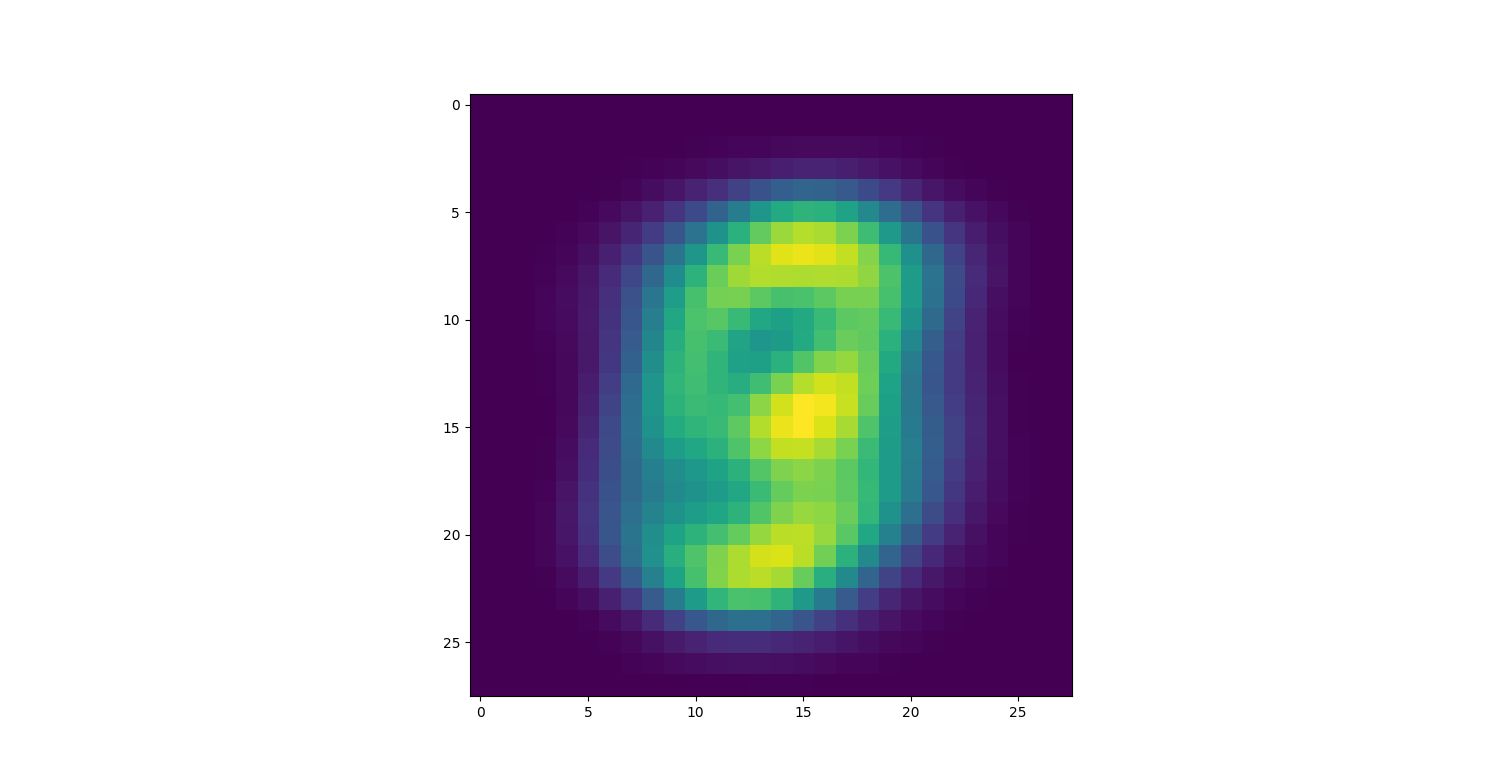
\includegraphics[width=0.70\paperwidth]{images/plot0.png}
            \caption{Mean value of all pixels in MNIST data set}
            \label{fig:mean}
        \end{figure}

        \part % b
        Log loss for multiclass classification is defined as
        \begin{align}
            \ell (w;x, y) & = -\log p(y \vert x) \nonumber                                                             \\
                          & = -\log \frac{\exp(w^\top_y x)}{\sum_{y' \in \{0, \dots,9\}}\exp(w^\top_{y'} x)} \nonumber \\
                          & = -w^\top_y x + \log \sum_{y' \in \{0, \dots , 9\}} \exp(w^\top_{y'} x)
        \end{align}

        The gradient of the log loss function is

        \setlength{\jot}{12pt}

        when $y = \tilde{y}$,
        \begin{align*}
            \nabla_{w_{\tilde{y}}} \ell & = \frac{\partial}{\partial w_{\tilde{y}}}\left( -w^\top_{\tilde{y}} x + \log \sum_{y' \in \{0, \dots , 9\}} \exp(w^\top_{y'} x)\right)                                                                                                                                         \\
                                        & = \frac{\partial}{\partial w_{\tilde{y}}}\left( -w^\top_{\tilde{y}} x \right) + \frac{\partial}{\partial w_{\tilde{y}}}\left(\log \sum_{y' \in \{0, \dots , 9\}} \exp(w^\top_{y'} x)\right)                                                                                    \\
                                        & = -x + \frac{\partial}{\partial w_{\tilde{y}}}\left(\log \sum_{y' \in \{0, \dots , 9\}} \exp(w^\top_{y'} x)\right)                                                                                                                                                             \\
                                        & = -x + \frac{1}{\sum_{y' \in \{0, \dots , 9\}} \exp(w^\top_{y'} x)} \frac{\partial}{\partial w_{\tilde{y}}}\left(\sum_{y' \in \{0, \dots , 9\}} \exp(w^\top_{y'} x)\right)                                                                                                     \\
                                        & = -x + \frac{1}{\sum_{y' \in \{0, \dots , 9\}} \exp(w^\top_{y'} x)} \frac{\partial}{\partial w_{\tilde{y}}}\left(\exp(w^\top_{\tilde{y}} x) + \sum_{y' \in \{0, \dots , 9\}, y' \neq \tilde{y}} \exp(w^\top_{y'} x)\right)                                                     \\
                                        & = -x + \frac{1}{\sum_{y' \in \{0, \dots , 9\}} \exp(w^\top_{y'} x)} \frac{\partial}{\partial w_{\tilde{y}}}\left(\exp(w^\top_{\tilde{y}} x)\right) + \frac{\partial}{\partial w_{\tilde{y}}}\left(\sum_{y' \in \{0, \dots , 9\}, y' \neq \tilde{y}} \exp(w^\top_{y'} x)\right) \\
                                        & = -x + \frac{\frac{\partial}{\partial w_{\tilde{y}}}\left(\exp(w^\top_{y'} x)\right)}{\sum_{y' \in \{0, \dots , 9\}} \exp(w^\top_{y'} x)}                                                                                                                                      \\
                                        & = -x + \frac{\exp(w^\top_{\tilde{y}} x)\frac{\partial}{\partial w_{\tilde{y}}}\left(w^\top_{\tilde{y}} x\right)}{\sum_{y' \in \{0, \dots , 9\}} \exp(w^\top_{y'} x)}                                                                                                           \\
                                        & = -x + \frac{\exp(w^\top_{\tilde{y}} x)x}{\sum_{y' \in \{0, \dots , 9\}} \exp(w^\top_{y'} x)}                                                                                                                                                                                  \\
                                        & = x\left(\frac{\exp(w^\top_{\tilde{y}} x)}{\sum_{y' \in \{0, \dots , 9\}} \exp(w^\top_{y'} x)} - 1\right)                                                                                                                                                                      \\
                                        & = x\left(\exp \left( \log \left(\frac{\exp(w^\top_{\tilde{y}}x)}{\sum_{y' \in \{0, \dots , 9\}} \exp(w^\top_{y'} x)}\right)\right) - 1\right)                                                                                                                                  \\
            \nabla_{w_{\tilde{y}}} \ell & = x\left(\exp \left(-\ell(w_{\tilde{y}} ; x, \tilde{y})\right) - 1\right)
        \end{align*}
        when $y \neq \tilde{y}$,
        \begin{align*}
            \nabla_{w_{\tilde{y}}} \ell & = \frac{\partial}{\partial w_{\tilde{y}}}\left( -w^\top_{y} x + \log \sum_{y' \in \{0, \dots , 9\}} \exp(w^\top_{y'} x)\right)                                                                                                                                            \\
                                        & = \frac{\partial}{\partial w_{\tilde{y}}}\left( -w^\top_{y} x \right) + \frac{\partial}{\partial w_{\tilde{y}}}\left(\log \sum_{y' \in \{0, \dots , 9\}} \exp(w^\top_{y'} x)\right)                                                                                       \\
                                        & = \frac{\partial}{\partial w_{\tilde{y}}}\left(\log \sum_{y' \in \{0, \dots , 9\}} \exp(w^\top_{y'} x)\right)                                                                                                                                                             \\
                                        & = \frac{1}{\sum_{y' \in \{0, \dots , 9\}} \exp(w^\top_{y'} x)} \frac{\partial}{\partial w_{\tilde{y}}}\left(\sum_{y' \in \{0, \dots , 9\}} \exp(w^\top_{y'} x)\right)                                                                                                     \\
                                        & = \frac{1}{\sum_{y' \in \{0, \dots , 9\}} \exp(w^\top_{y'} x)} \frac{\partial}{\partial w_{\tilde{y}}}\left(\exp(w^\top_{\tilde{y}} x) + \sum_{y' \in \{0, \dots , 9\}, y' \neq \tilde{y}} \exp(w^\top_{y'} x)\right)                                                     \\
                                        & = \frac{1}{\sum_{y' \in \{0, \dots , 9\}} \exp(w^\top_{y'} x)} \frac{\partial}{\partial w_{\tilde{y}}}\left(\exp(w^\top_{\tilde{y}} x)\right) + \frac{\partial}{\partial w_{\tilde{y}}}\left(\sum_{y' \in \{0, \dots , 9\}, y' \neq \tilde{y}} \exp(w^\top_{y'} x)\right) \\
                                        & = \frac{\frac{\partial}{\partial w_{\tilde{y}}}\left(\exp(w^\top_{y'} x)\right)}{\sum_{y' \in \{0, \dots , 9\}} \exp(w^\top_{y'} x)}                                                                                                                                      \\
                                        & = \frac{\exp(w^\top_{\tilde{y}} x)\frac{\partial}{\partial w_{\tilde{y}}}\left(w^\top_{\tilde{y}} x\right)}{\sum_{y' \in \{0, \dots , 9\}} \exp(w^\top_{y'} x)}                                                                                                           \\
                                        & = \frac{\exp(w^\top_{\tilde{y}} x)x}{\sum_{y' \in \{0, \dots , 9\}} \exp(w^\top_{y'} x)}                                                                                                                                                                                  \\
                                        & = x\exp \left( \log \left(\frac{\exp(w^\top_{\tilde{y}} x)}{\sum_{y' \in \{0, \dots , 9\}} \exp(w^\top_{y'} x)}\right)\right)                                                                                                                                             \\
            \nabla_{w_{\tilde{y}}} \ell & = x\exp \left(-\ell(w_{\tilde{y}} ; x, \tilde{y})\right)
        \end{align*}

        \setlength{\jot}{3pt}

        \newpage

        \part % c

        \begin{figure}[!ht]
            \centering
            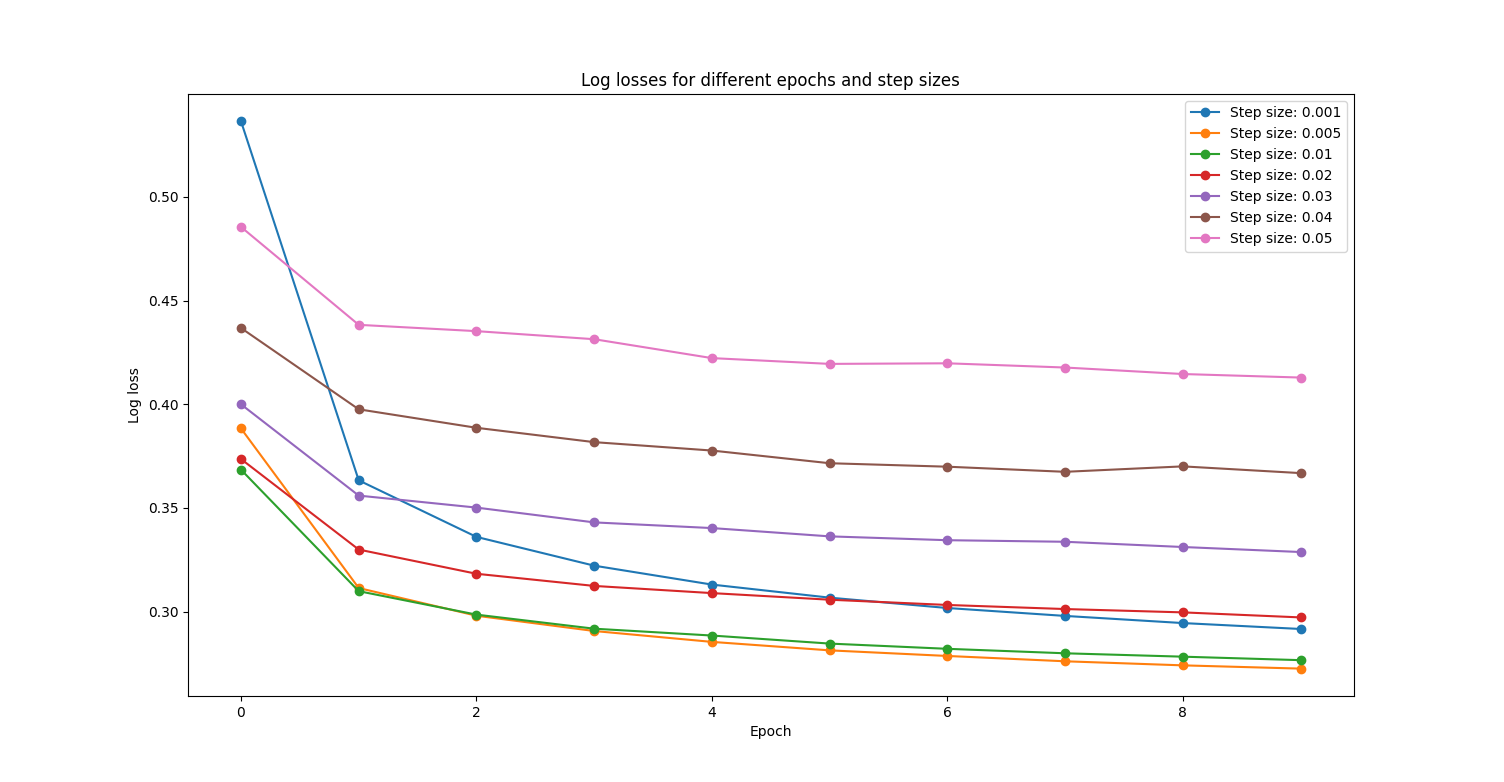
\includegraphics[width=0.70\paperwidth]{images/plot1.png}
            \caption{Log loss curves for different step sizes}
            \label{fig:log-loss}
        \end{figure}

        The plot seen in figure \ref{fig:log-loss} shows the average log-loss curve for a set of step sizes. It is clear that some step sizes seem to be converging towards a lower log loss than others over time, but they all
        have the shape of an exponential decay curve. The general trend seems to be that the higher the step size, the higher the final epoch's loss. With larger step sizes, the changes in $w$ can be too large and the change would
        skip over the local minimum while never entering the minimum. However, is the step size is smaller than 0.005, the loss also increases due to the fact that more epochs are required to find the lower minimum value. Therefore,
        with 10 epochs and 60,000 data points, a step size $\approx 0.005$ would give the lowest log-loss. This is a similar case with the zero-one loss as shown in \ref{fig:zero-one-loss}, where the higher the step size, the higher
        the zero-one loss with a minmum zero-one loss given by the step size of 0.005.

        After training a classifier with 10 epochs and a step size of 0.005, the final zero-one loss was $\approx 0.075$, or a $7.5\%$ misclassification rate.

    \end{parts}
\end{questions}

\newpage
\section*{Appendix}

\begin{figure}[!ht]
    \centering
    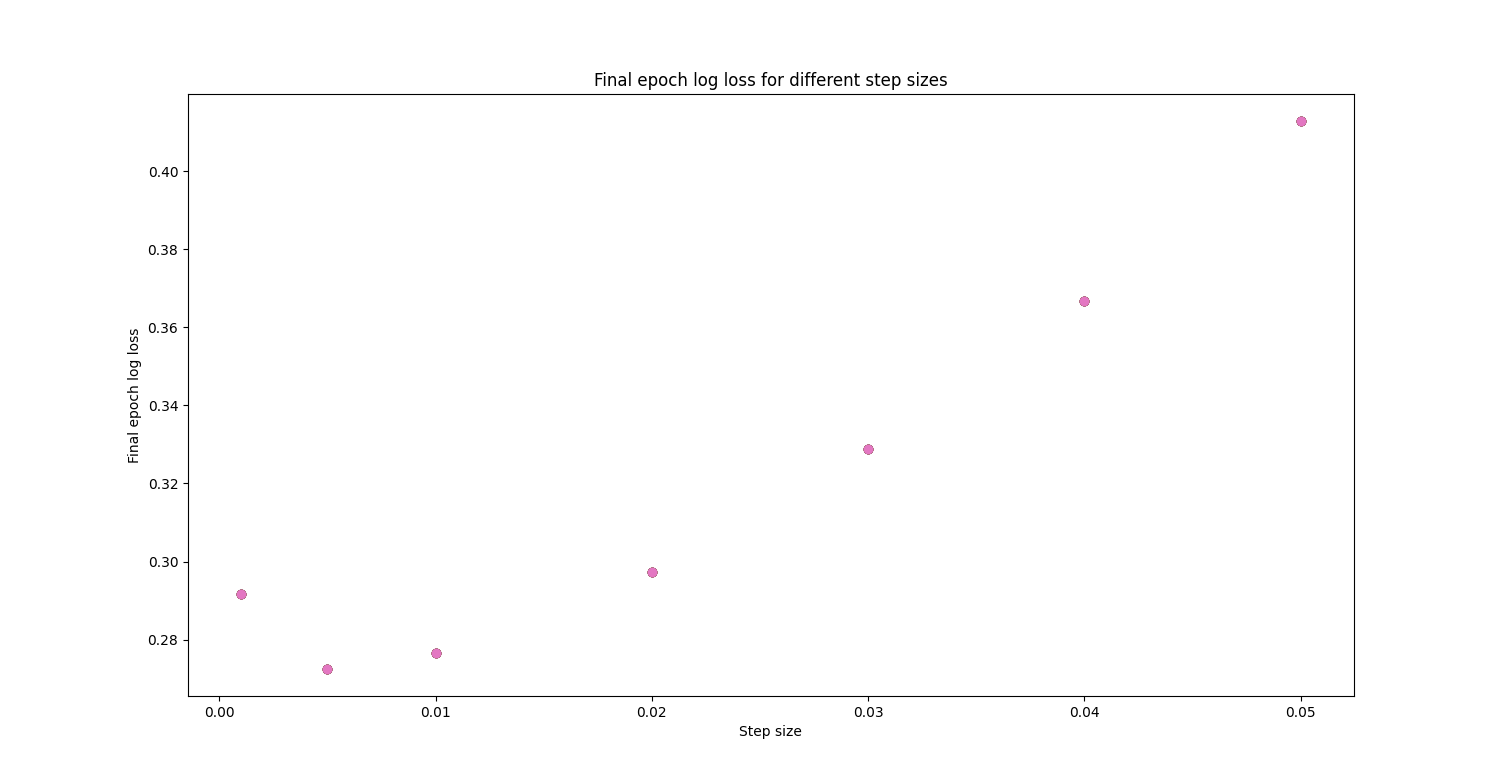
\includegraphics[width=0.70\paperwidth]{images/plot3.png}
    \caption{Final epoch log loss for different step sizes}
    \label{fig:final-log-loss}
\end{figure}

\begin{figure}[!ht]
    \centering
    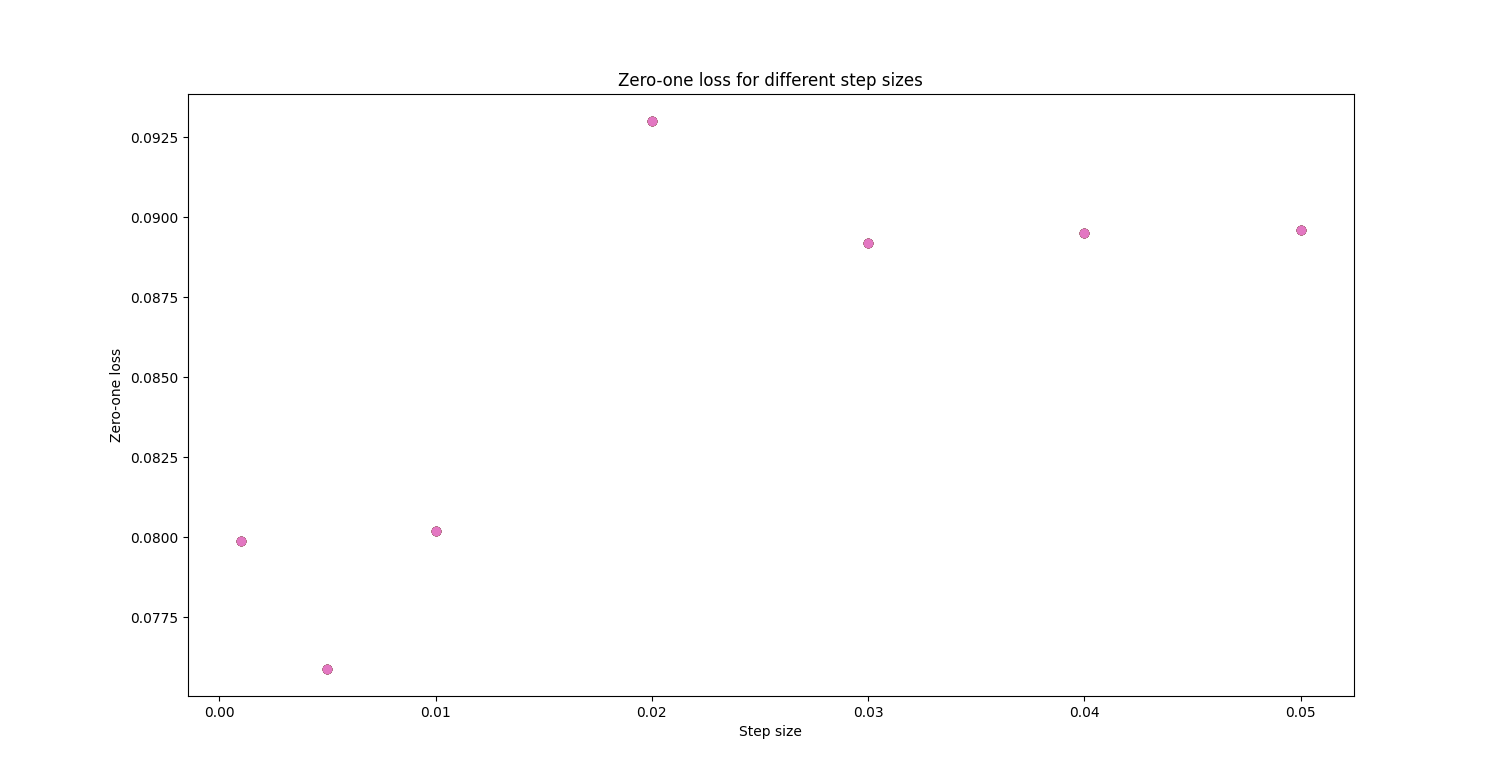
\includegraphics[width=0.70\paperwidth]{images/plot2.png}
    \caption{Zero-one loss for different step sizes}
    \label{fig:zero-one-loss}
\end{figure}

\newpage

\begin{python}
    import numpy as np
    import matplotlib.pyplot as plt
    import mnist
    import logging
    from time import time


    class SGDMnistClassifier:
        def __init__(self, xs: np.ndarray, ys: np.ndarray):
            self.data = list(zip(xs, ys))
            self.w = np.zeros((10, xs.shape[1]))

        def zero_one_loss(self, xs: np.ndarray, ys: np.ndarray):
            """
            Calculate the zero-one loss of the classifier on the given data.
            """
            correct = 0
            for x, y in list(zip(xs, ys)):
                correct += self.classify(x) == y
            return 1 - correct / len(xs)

        def shuffle(self):
            """
            Shuffles the data in place.
            """
            if self.data is None:
                raise ValueError("No data to shuffle.")
            np.random.shuffle(self.data)

        def p(self, x: np.ndarray, y: np.uint8) -> np.float64:
            """
            Calculate the probability of x being in class y.
            """
            return np.exp(self.w[y] @ x) / np.sum(np.exp(self.w @ x))

        def classify(self, x: np.ndarray):
            """
            Return the class of x with the highest probability.
            """
            return np.argmax([np.dot(x, self.w[y]) for y in range(10)])

        def loss(self, x: np.ndarray, y: np.uint8):
            """
            Returns the log loss
            """
            return -self.w[y] @ x + np.logaddexp.reduce(self.w @ x)

        def dloss(self, x: np.ndarray, y: np.uint8, y_true: np.uint8):
            """
            Returns the gradient of the loss function with respect to the weights.
            """
            if y != y_true:
                return x * (np.exp(-self.loss(x, y)))
            return x * (np.exp(-self.loss(x, y)) - 1)

        def learn(self, step_size, epochs):
            """
            Train the classifier using stochastic gradient descent.
            """
            if self.data is None:
                raise ValueError("No data to learn from.")

            losses = np.empty(epochs)

            for e in range(epochs):
                loss_values = []
                self.shuffle()
                logging.info(f"Epoch {e + 1} of {epochs}...")
                for x_i, y_i in self.data:
                    loss_values.append(self.loss(x_i, y_i))
                    for y_j in range(10):
                        self.w[y_j] -= step_size * self.dloss(x_i, np.uint8(y_j), y_i)

                losses[e] = np.mean(loss_values)

            return losses


    def part_a():
        images = mnist.load_images("data/train-images-idx3-ubyte")
        reshaped_images = np.array([np.reshape(im, (784,)) for im in images])
        mean_image = np.reshape(np.mean(reshaped_images, axis=0), (28, 28))
        _, ax = plt.subplots()
        ax.imshow(mean_image)
        plt.show(block=False)


    def part_c():
        start_time = time()

        # Load training data
        training_images = mnist.load_images("data/train-images-idx3-ubyte")
        training_images = np.array([np.reshape(im, (784,)) / 255 for im in training_images])
        training_labels = mnist.load_labels("data/train-labels-idx1-ubyte")

        # Load testing data
        testing_images = mnist.load_images("data/t10k-images-idx3-ubyte")
        testing_images = np.array([np.reshape(im, (784,)) / 255 for im in testing_images])
        testing_labels = mnist.load_labels("data/t10k-labels-idx1-ubyte")

        # Initialise data
        step_sizes = [
            0.001,
            0.005,
            0.01,
            0.02,
            0.03,
            0.04,
            0.05,
        ]
        log_losses_epoch = np.empty(len(step_sizes), dtype=list)
        log_losses = np.empty(len(step_sizes), dtype=np.float64)
        zero_one_losses = np.empty(len(step_sizes), dtype=np.float64)

        # Collect data
        for i, step_size in enumerate(step_sizes):
            epoch_time = time()
            classifier = SGDMnistClassifier(training_images, training_labels)
            logging.info(
                f"Learning with step size {step_size} ({i + 1}/{len(step_sizes)})..."
            )
            log_losses_epoch[i] = classifier.learn(step_size, epochs=10)
            log_losses[i] = log_losses_epoch[i][-1]
            zero_one_losses[i] = classifier.zero_one_loss(testing_images, testing_labels)
            logging.info(f"Done in {np.round(time() - epoch_time, decimals=2)} seconds")

        logging.info(f"Total time: {np.round(time() - epoch_time, decimals=2)} seconds")

        # Plot data
        _, ax = plt.subplots()
        for i, step_size in enumerate(step_sizes):
            ax.plot(log_losses_epoch[i], label="Step size: " + str(step_size), marker="o")
        ax.legend()
        ax.set_xlabel("Epoch")
        ax.set_ylabel("Log loss")
        ax.set_title("Log losses for different epochs and step sizes")

        _, ax = plt.subplots()
        for i, step_size in enumerate(step_sizes):
            ax.scatter(step_sizes, log_losses)
        ax.set_xlabel("Step size")
        ax.set_title("Final epoch log loss for different step sizes")
        ax.set_ylabel("Final epoch log loss")

        _, ax = plt.subplots()
        for i, step_size in enumerate(step_sizes):
            ax.scatter(step_sizes, zero_one_losses)
        ax.set_xlabel("Step size")
        ax.set_ylabel("Zero-one loss")
        ax.set_title("Zero-one loss for different step sizes")

        # Train with best step size
        step_size = 0.01
        logging.info(f"Learning with step size {step_size} (final)...")
        classifier = SGDMnistClassifier(training_images, training_labels)
        classifier.learn(0.01, epochs=10)

        # Test classifier
        zero_one_loss = classifier.zero_one_loss(training_images, training_labels)
        logging.info(f"Zero-one loss on test set: {zero_one_loss}")


    def main():
        np.seterr(all="raise")
        logging.basicConfig(level=logging.INFO, format="[%(levelname)s] %(message)s")
        part_a()
        part_c()
        plt.show()


    if __name__ == "__main__":
        main()
\end{python}


\end{document}